\documentclass[a4j,twocolumn,uplatex]{jsarticle}

\def\Vec#1{\mbox{\boldmath $#1$}}
\usepackage[dvipdfmx]{graphicx}

\setlength{\textheight}{275mm}
\headheight 5mm
\topmargin -30mm
\textwidth 185mm
\oddsidemargin -15mm
\evensidemargin -15mm
\pagestyle{empty}

\begin{document}
\title{GitHubを利用したRuby初心者支援ソフトの開発}
\author{情報科学科 西谷研究室 2549 浦田 航貴}
\date{}
\maketitle
\section{1 はじめに}
西谷研究室に在籍している学生は,Rubyプログラミングを修得するために初心者向けの問題集を使って学習している.本研究は進捗状況の管理や指導者からの添削をより容易におこなえるように改善するため,バージョン管理ソフトGitHubを利用することにした.さらにRubyプログラミングで重要となるテスト駆動をおこなえる環境を用意する.これにより,学習者自身が出力チェックできるようにしRubyプログラミングにおけるテスト実行に自然と慣れるような学習形態を目指す.本研究はRuby初心者が文法だけでなく,Rubyプログラミングにおける振舞いを身につけるための支援ソフトを開発する.

\section{2 使用ツール}
\subsection{2.1 GitHubについて}
GitHubは,コンピュータープログラムの元となるソースコードをインターネット上で管理するためのサービスである.複数人が携わるソフトウェア開発において,ソースコードの共有や,バージョン管理といった作業は必要不可欠となる.

またソースコードを始めとするプログラム開発に必要なファイルやそれらの変更履歴等を保存する「リポジトリ」と呼ばれる場所があり,ソースコード等のバージョンを管理する機能の他,プログラム開発等に対する開発者間でのレビューやコメント機能,プログラム開発の進捗を管理する機能等が備わっている.[1]

\subsection{2.2 RSpecについて}
RSpecは,プログラムの振舞いを記述するためのドメイン特化言語を提供するフレームワークであり,「プログラムの振舞い」とはプログラム全体あるいは様々なレベルでの部分 (モジュールやクラス,メソッド) に対して期待する振舞いのことである.またドメイン特化言語 (Domain Specific Language:DSL) は,特定の問題領域 (ドメイン) を記述するために設計された言語である.[2]

Rspecによって期待されている値と出力している値が一致しているかを確認できる.テストコードを使えば「puts を使って毎回目視で確認」なんてするよりも,高速で確実に実行結果を検証することができる.また,テストコードを書いておけば他の人も「このメソッドを呼ぶと何が起こるか」を理解しやすくなる.

\section{開発要件}
本研究における開発要件は以下の通りである.

\subsection{GitHubでの進捗確認}
本研究ではGithubを使用し,進捗状況の管理や指導者からの添削をより容易できるようにする.また緑の濃さに応じて進捗状況を把握でき,作業した日時と作業内容も確認できる.

\begin{center}
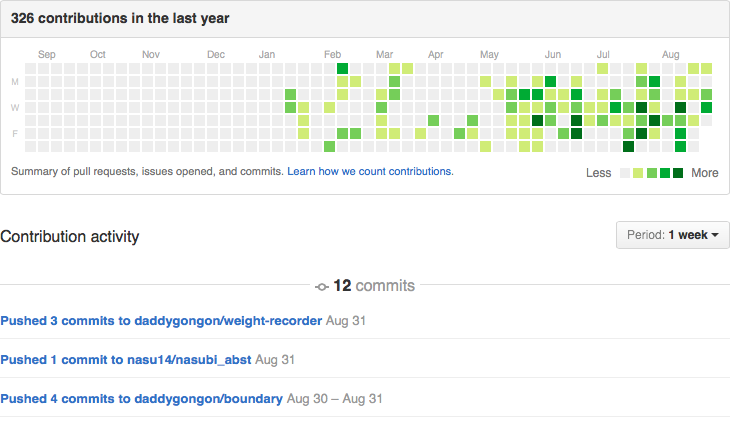
\includegraphics[width=9cm]{GitHub.jpg}
\end{center}

この特徴を利用する事で,チーム開発の手法を修得できる.\\

\subsection{テスト駆動(RSpec→Test::Unit)}
現段階,西谷研究室に在籍している学生はテストする時,RSpecを使用している.RSpecは,独自のDSL(ドメイン固有言語)を使っているために学習コストが大きいと感じた.

また初心者として私自身がRSpecを使用したところ,少しの間違いでもエラーが複雑に表示されることや,すぐにエラーを理解するということが困難であった.より単純でわかりやすい結果を出力してくれるTest::Unit(minitest)を用いることを考えている.

\section{結論と今後の課題}


\section{参考文献}
[1]「GitHub」,横田一輝\\ ~~~~~~~ https://kotobank.jp/word/GitHub-1725201
\newline ~~~[2]「Rubyst Magazine」, かくたに もろはし vol.54\\~~~~~~~~http://magazine.rubyist.net/?0021-Rspec

\end{document}
